\chapter{Introduction}
\label{cap:introducao}

This chapter presents the context of the work described in this dissertation, the problem that
motivates it, the research questions and the objectives defined, the scientific contributions and
the organisation of the document.

\section{Context}
\label{sec:intro_origem}

Buying shares has become a low-friction operation, available through mobile applications and
without significant brokerage costs. Most adults in the United States now hold shares, directly or
through funds and retirement plans \autocite{gallup2025stock}, in a market whose capitalisation
exceeds 62 trillion US dollars \autocite{sifma2025factbook}, as shown in
Figure~\ref{fig:mercado_eua}.

Ease of access has not extended, however, to the interpretation of information. When the price of
an asset moves, the retail investor has limited instruments for determining what that movement
means.

The behaviour of this segment is the object of current research, and two recent results delimit the
problem addressed in this dissertation. The first is that retail investor attention is today a
measured quantity, whose indicators are discussed and compared in the literature
\autocite{cahill2025attention}: what determines what the investor observes is studied as a
variable, and not as chance. The second is that retail participation in the market, and the
conditions under which it trades, remain the subject of active review
\autocite{ernst2026retail}. Chapter~\ref{cap:contexto} develops the behavioural mechanisms that
this literature documents, and which explain why the absence of context is more costly to this
audience than to a professional.

What matters to retain from this body of work is what delimits the problem. The signals that
capture the investor's attention arrive without context, and the decision that follows is taken
under conditions the literature documents as unfavourable. Three concrete questions remain
unanswered at the moment the investor observes a price movement:

\begin{enumerate}
  \item \textbf{is the movement unusual?} A four per cent change is a rare event in a low
        volatility company and an ordinary day in a volatile one;
  \item \textbf{does the movement originate in the company or in the market?} A fall that follows
        the market and an isolated fall are distinct situations;
  \item \textbf{are there precedents, and what was their outcome?} The existence of comparable
        days in the past, and of what followed them, allows the observed movement to be situated.
\end{enumerate}

Current free applications display the percentage change and answer none of the three. There are
recent products that claim to go further, and Section~\ref{sec:ctx_ferramentas} names them: what
their own pages describe is a summary in natural language, and not individual past cases with the
outcome measured. Professional financial information terminals do answer all three, and are
not available free of charge or at a cost accessible to the investor profile in question. The gap does not follow
from the unavailability of data, which exist in quantity and are free, but from the absence of
verifiable context built on them.

\begin{figure}[ht]
\centering
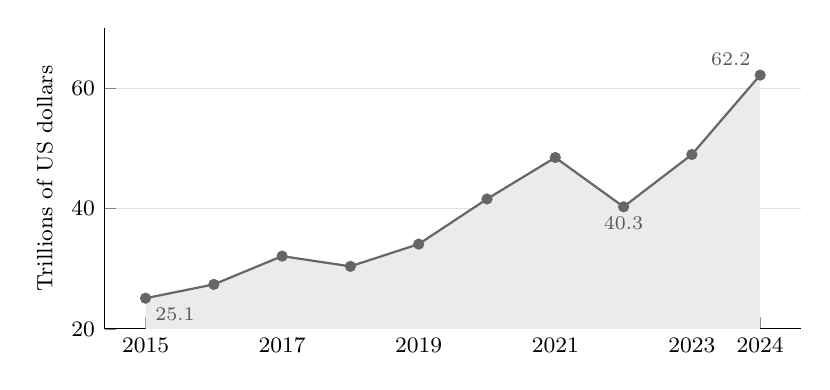
\begin{tikzpicture}
\begin{axis}[
  % Time series: the shape is the line, not the bar. Ten bars labelled one by one competed
  % with the reading that matters, which is the trajectory and the 2022 break.
  width=0.86\textwidth, height=5.4cm,
  ymin=20, ymax=70, xmin=2014.4, xmax=2024.6,
  xtick={2015,2017,2019,2021,2023,2024},
  % years do NOT take a thousands separator: without this pgfplots writes 2,015.
  xticklabel style={/pgf/number format/.cd, fixed, 1000 sep={}},
  ylabel={Trillions of US dollars},
  tick label style={font=\footnotesize}, label style={font=\footnotesize},
  ymajorgrids, grid style={black!12}, axis lines*=left,
  ]
  \addplot[draw=none, fill=black!8, forget plot] coordinates {
    (2015,20) (2015,25.1) (2016,27.4) (2017,32.1) (2018,30.4) (2019,34.1)
    (2020,41.6) (2021,48.5) (2022,40.3) (2023,49.0) (2024,62.2) (2024,20)} \closedcycle;
  \addplot[black!60, thick, mark=*, mark size=1.6pt,
           mark options={fill=black!60, draw=none}] coordinates {
    (2015,25.1) (2016,27.4) (2017,32.1) (2018,30.4) (2019,34.1)
    (2020,41.6) (2021,48.5) (2022,40.3) (2023,49.0) (2024,62.2)};
  % only the three points the prose invokes: the start, the break, and the end.
  \node[font=\scriptsize, black!65, below right] at (axis cs:2015,25.1) {25.1};
  \node[font=\scriptsize, black!65, below] at (axis cs:2022,40.3) {40.3};
  \node[font=\scriptsize, black!65, above left] at (axis cs:2024,62.2) {62.2};
\end{axis}
\end{tikzpicture}
\caption[Capitalisation of the United States stock market]{Capitalisation of the United States
stock market, 2015--2024, in trillions of US dollars. Compiled from the data of the SIFMA Capital
Markets Fact Book \autocite{sifma2025factbook}.}
\label{fig:mercado_eua}
\end{figure}

\section{Problem description}
\label{sec:intro_sistema}

This dissertation presents InvestiGator, a financial alerting system built exclusively on free data
sources, which monitors a set of companies, detects events that depart from the usual behaviour of
each one, and issues alerts accompanied by the explanation and the evidence that support them.

The system has two triggers, shown in Figure~\ref{fig:conceito}: a price movement that is unusual
for the company in question, or the arrival of a relevant news item about it. In both cases, the
message delivered identifies the event, the criterion by which it was considered unusual, the
provenance of the data used, and the semantically closest past cases, with the observed behaviour
of the price after each of them.

One design decision runs through the system and conditions all the others: \textbf{the system does
not produce price forecasts}. It does not indicate future direction, does not issue buy or sell
recommendations, and does not present price targets. This restriction has two justifications. The
first is verifiability: a statement about a past event can be confirmed against the record at the
moment it is read, whereas a forecast can only be assessed after the investor's decision has
already been taken. The second is theoretical: the efficient market hypothesis, in its semi-strong
form, makes the systematic anticipation of movements from publicly available information
improbable. Chapter~\ref{cap:contexto} develops it and identifies the corresponding literature.
This dissertation does not test that hypothesis, nor does it rely on it to establish any
conclusion.

\begin{figure}[ht]
\centering
\begin{tikzpicture}[
  font=\small, >={Stealth[length=2.2mm]},
  gat/.style={draw, rounded corners, fill=black!8, align=center, text width=3.1cm, minimum height=1cm},
  sis/.style={draw, rounded corners, fill=black!3, align=center, text width=2.6cm, minimum height=1.6cm},
  saida/.style={draw, rounded corners, fill=black!3, align=center, text width=3.8cm, minimum height=1.6cm},
]
  \node[gat] (g1) {unusual price\\ movement};
  \node[gat, below=7mm of g1] (g2) {relevant news\\ about the company};
  \node[sis] (sis) at ($(g1)!0.5!(g2) + (3.9,0)$) {\textbf{InvestiGator}};
  \node[saida, right=1.3cm of sis] (out) {explained alert\\[2pt]
    \footnotesize what happened\\ \footnotesize why · sources\\ \footnotesize precedents};
  \node[right=1.0cm of out, align=center] (inv) {\footnotesize investor};
  \draw[->] (g1) -- (sis);
  \draw[->] (g2) -- (sis);
  \draw[->] (sis) -- (out);
  \draw[->] (out) -- (inv);
\end{tikzpicture}
\caption[The two triggers of the system]{The two triggers of the system and the output they
produce. The investor receives an alert accompanied by the evidence that allows it to be verified,
and not merely the notification that the price has moved.}
\label{fig:conceito}
\end{figure}

\section{Objectives and research questions}
\label{sec:intro_objetivos}

The general objective of this dissertation is to design, build and evaluate an explainable
financial alerting system for retail investors, using exclusively free data sources.

Three research questions follow from this objective, each associated with a measurement and a
success criterion defined before the experiments were carried out:
% The long form of the acronym is dispensed with here: the preceding sentence spells it out,
% and `\gls{QI}1` on first use would print 'Research Question (RQ)1', with the number glued
% to the closing bracket. The acronym still appears in the List of Acronyms, because the
% later `\gls` uses go on recording it.
\glsunset{QI}
\begin{itemize}
  \item \textbf{\gls{QI}1, detection.} Can a simple and transparent statistical method detect
        unusual movements consistently across companies with distinct volatilities, and do so
        better than a fixed threshold rule?
  \item \textbf{\gls{QI}2, precedents.} Can the system retrieve past news from another company in
        the same sector better than trivial alternatives, and measure the subsequent behaviour of
        the price without resorting to information posterior to the moment of the query?
  \item \textbf{\gls{QI}3, triage.} Can a trained model decide which news items justify an alert
        better than a baseline built only on volatility?
\end{itemize}

The investor's second question, concerning the separation between the market component and the
company-specific component, is addressed by a technique described in
Chapter~\ref{cap:metodologia} but does not give rise to a research question. The reason is
methodological: the split of a movement has no observable reference value against which it can be
compared, since that quantity exists only relative to a model.
Section~\ref{sec:av_decomposicao} establishes what, in spite of that, remains measurable in the
technique.

These questions take the form of four objectives:

\begin{enumerate}
  \item to build the complete system, from data acquisition to the delivery of the alert;
  \item to evaluate each component against transparent baselines;
  \item to ensure that the explanations presented are faithful to what the system computed;
  \item to report the results obtained, including those that do not confirm the initial
        expectations.
\end{enumerate}

\section{Scientific contributions}
\label{sec:intro_contribuicoes}

This being a dissertation in \gls{AI} Engineering, the contribution does not lie in the formulation
of a new algorithm, but in the selection, integration and critical evaluation of established
techniques until they constitute a working, explainable and reproducible system. Four
contributions are identified:

\begin{enumerate}
  \item \textbf{A complete system in operation}, with both triggers, built on free sources and
        actually deployed, and not a laboratory demonstration.
  \item \textbf{A reproducible method for measuring the behaviour of the price following
        semantically close news items}, combining retrieval by sentence similarity with event
        study windows, without using information posterior to the moment of the decision.
        Chapter~\ref{cap:contexto} identifies the two lines of work from which they come.
  \item \textbf{A purpose-built dataset and a model trained on it}, with 79{,}753 examples
        constructed from the public \gls{FNSPID} corpus \autocite{dong2024fnspid} and from price
        series, with the model, the calibration and the metrics kept as versioned artefacts.
  \item \textbf{An evaluation of each component against transparent baselines}, including the
        result that contradicts the initial hypothesis, reported as such.
\end{enumerate}

\section{Structure of the document}
\label{sec:intro_estrutura}

Chapter~\ref{cap:contexto} presents the state of the art, characterising the target audience, the
tools currently available and the technical areas from which the components used are drawn.
Chapter~\ref{cap:metodologia} describes the data and the four techniques that constitute the
system. Chapter~\ref{cap:sistema} describes the architecture of InvestiGator and the path of a news
item from collection to delivery. Chapter~\ref{cap:avaliacao} presents the experimental design and
the results obtained for each research question. Chapter~\ref{cap:conclusoes} synthesises the
answers, identifies the limitations of the work and sets out the lines of future development.

Each mechanism described is illustrated on a real case, with the values actually computed by the
system, and not on examples constructed for the purpose.

% ⚠️ THE PARAGRAPH ON THE LANGUAGE CONVENTION WAS REMOVED HERE, AND ITS ABSENCE IS DELIBERATE.
% In the Portuguese tree the prose is Portuguese and the interior of the figures is English, and
% that chapter states why. In this tree both are English, so the paragraph would explain a
% divergence that does not exist.
%
% This comment used to predict that the paragraph would be removed from the Portuguese
% tree once its figures were converted. The figures were converted on 2026-09-06 and the
% paragraph was REWRITTEN, not removed, because two categories of material stay in English
% there for reasons that survive the conversion: the quoted news headlines, whose corpus is
% English and whose correspondence with the source would break under translation, and the
% screenshots, whose interface is English by product decision. Neither needs stating here,
% where the whole document is English.
